\documentclass[12pt,a4paper]{article}

% ─── Packages ────────────────────────────────────────────────────────────────
\usepackage[top=2.5cm, bottom=2.5cm, left=2.8cm, right=2.8cm]{geometry}
\usepackage[T1]{fontenc}
\usepackage[utf8]{inputenc}
\usepackage{xcolor}
\usepackage{graphicx}
\usepackage{booktabs}
\usepackage{array}
\usepackage{tabularx}
\usepackage{multirow}
\usepackage{amsmath}
\usepackage{listings}
\usepackage{fancyhdr}
\usepackage{titlesec}
\usepackage{tocloft}
\usepackage{hyperref}
\usepackage{mdframed}
\usepackage{enumitem}
\usepackage{caption}
\usepackage{float}
\usepackage{colortbl}
\usepackage{tikz}
\usepackage{pgfplots}
\pgfplotsset{compat=1.18}

% ─── Colour Palette ──────────────────────────────────────────────────────────
\definecolor{primaryblue}{RGB}{0, 74, 127}
\definecolor{accentblue}{RGB}{0, 120, 210}
\definecolor{lightblue}{RGB}{220, 237, 252}
\definecolor{darkgray}{RGB}{50, 50, 50}
\definecolor{medgray}{RGB}{120, 120, 120}
\definecolor{lightgray}{RGB}{245, 245, 245}
\definecolor{codegreen}{RGB}{40, 140, 70}
\definecolor{codepurple}{RGB}{130, 40, 160}
\definecolor{codebrown}{RGB}{160, 80, 0}
\definecolor{sectionrule}{RGB}{0, 100, 180}
\definecolor{placeholderbg}{RGB}{255, 251, 230}
\definecolor{placeholderborder}{RGB}{200, 160, 0}
\definecolor{subseccolor}{RGB}{0, 90, 160}

% ─── Hyperref Setup ──────────────────────────────────────────────────────────
\hypersetup{
  colorlinks = true,
  linkcolor  = primaryblue,
  urlcolor   = accentblue,
  citecolor  = primaryblue,
  pdftitle   = {DAS 839 Assignment II Report},
  pdfauthor  = {Group},
}

% ─── Section Formatting ──────────────────────────────────────────────────────
\titleformat{\section}
  {\large\bfseries\color{primaryblue}}
  {\thesection}{1em}{}
  [\vspace{-0.3em}\color{sectionrule}\rule{\linewidth}{1.5pt}\vspace{0.3em}]

\titleformat{\subsection}
  {\normalsize\bfseries\color{subseccolor}}
  {\thesubsection}{1em}{}

\titleformat{\subsubsection}
  {\normalsize\itshape\color{darkgray}}
  {\thesubsubsection}{1em}{}

\titlespacing*{\section}{0pt}{1.6em}{0.6em}
\titlespacing*{\subsection}{0pt}{1.2em}{0.4em}
\titlespacing*{\subsubsection}{0pt}{0.9em}{0.3em}

% ─── Header / Footer ─────────────────────────────────────────────────────────
\pagestyle{fancy}
\fancyhf{}
\fancyhead[L]{\small\color{medgray}\textbf{DAS 839 -- NoSQL Systems}}
\fancyhead[R]{\small\color{medgray}Assignment II Report}
\fancyfoot[C]{\small\color{medgray}\thepage}
\renewcommand{\headrulewidth}{0.4pt}
\renewcommand{\footrulewidth}{0pt}
\renewcommand{\headrule}{\hbox to\headwidth{\color{sectionrule}\leaders\hrule height \headrulewidth\hfill}}

% ─── Code Listing Style ──────────────────────────────────────────────────────
\lstdefinestyle{javacode}{
  language=Java,
  basicstyle=\ttfamily\footnotesize,
  keywordstyle=\bfseries\color{primaryblue},
  commentstyle=\itshape\color{codegreen},
  stringstyle=\color{codebrown},
  numberstyle=\tiny\color{medgray},
  numbers=left,
  numbersep=8pt,
  stepnumber=1,
  showstringspaces=false,
  breaklines=true,
  breakatwhitespace=true,
  frame=single,
  framesep=4pt,
  rulecolor=\color{accentblue},
  backgroundcolor=\color{lightgray},
  xleftmargin=12pt,
  xrightmargin=4pt,
  captionpos=b,
  tabsize=2,
}

\lstdefinestyle{pseudocode}{
  basicstyle=\ttfamily\footnotesize,
  keywordstyle=\bfseries\color{primaryblue},
  commentstyle=\itshape\color{codegreen},
  numbers=none,
  showstringspaces=false,
  breaklines=true,
  frame=single,
  rulecolor=\color{medgray},
  backgroundcolor=\color{lightblue},
  xleftmargin=8pt,
  xrightmargin=4pt,
  tabsize=2,
  morekeywords={function,for,each,if,else,return,emit,end,Map,Reduce,in,do,while,output},
}

\lstdefinestyle{bashcode}{
  language=bash,
  basicstyle=\ttfamily\footnotesize,
  keywordstyle=\bfseries\color{accentblue},
  commentstyle=\itshape\color{codegreen},
  numbers=none,
  showstringspaces=false,
  breaklines=true,
  frame=single,
  rulecolor=\color{medgray},
  backgroundcolor=\color{lightgray},
  xleftmargin=8pt,
  tabsize=2,
}

% ─── Custom Environments ─────────────────────────────────────────────────────
% Placeholder box
\newmdenv[
  backgroundcolor=placeholderbg,
  linecolor=placeholderborder,
  linewidth=1.2pt,
  roundcorner=4pt,
  skipabove=8pt,
  skipbelow=8pt,
  innerleftmargin=10pt,
  innerrightmargin=10pt,
  innertopmargin=8pt,
  innerbottommargin=8pt,
]{placeholder}

% Info box
\newmdenv[
  backgroundcolor=lightblue,
  linecolor=accentblue,
  linewidth=1pt,
  roundcorner=4pt,
  skipabove=6pt,
  skipbelow=6pt,
  innerleftmargin=10pt,
  innerrightmargin=10pt,
  innertopmargin=6pt,
  innerbottommargin=6pt,
]{infobox}

% ─── Table of Contents Styling ───────────────────────────────────────────────
\renewcommand{\cftsecfont}{\bfseries\color{primaryblue}}
\renewcommand{\cftsecpagefont}{\bfseries\color{primaryblue}}
\renewcommand{\cftsubsecfont}{\color{darkgray}}
\setlength{\cftbeforesecskip}{4pt}

% ─── Misc Helpers ────────────────────────────────────────────────────────────
\newcommand{\phbox}[1]{%
  \begin{placeholder}
    \textcolor{codebrown}{\textbf{[PLACEHOLDER]}} \textit{#1}
  \end{placeholder}%
}

% Inline version safe inside tabular cells
\newcommand{\ph}[1]{\textcolor{placeholderborder}{\textit{\textbf{[}#1\textbf{]}}}}

\newcommand{\screenshotbox}{%
  \begin{placeholder}
    \textcolor{codebrown}{\textbf{[SCREENSHOT]}} \textit{Insert relevant screenshot here (execution time, output sample, Hadoop job summary, etc.)}
  \end{placeholder}%
}

% Runtime inline helper
\newcommand{\runtime}[3]{%
  \texttt{real~#1\quad user~#2\quad sys~#3}%
}

% ─────────────────────────────────────────────────────────────────────────────
\begin{document}

% ╔══════════════════════════════════════════════════════════╗
% ║                      TITLE PAGE                         ║
% ╚══════════════════════════════════════════════════════════╝
\begin{titlepage}
  \centering
  \vspace*{1.5cm}

  {\color{primaryblue}\rule{\linewidth}{2pt}}
  \vspace{0.4cm}

  {\Huge\bfseries\color{primaryblue} DAS 839 -- NoSQL Systems}\\[0.6em]
  {\LARGE\color{darkgray} Assignment II: MapReduce \& Apache Hadoop}

  \vspace{0.4cm}
  {\color{primaryblue}\rule{\linewidth}{2pt}}

  \vspace{2.5cm}

  \begin{minipage}{0.75\textwidth}
    \centering
    \large
    \begin{tabular}{rl}
      \textbf{Course}   & DAS 839 -- NoSQL Systems \\[4pt]
      \textbf{Group Members} & \ph{Siddharth Anil -- IMT2023503} \\
                        & \ph{Yash Gupta -- IMT2023125} \\
                        & \ph{Hitanshu Seth -- IMT2023100}\\
                        & \ph{Pranay Kelotra -- IMT2023563} \\[4pt]
      \textbf{Submitted} & \today \\
    \end{tabular}
  \end{minipage}

  \vfill

  \begin{infobox}
    \textbf{Submission Notes:} Run instructions are provided in \texttt{problem\_1.txt} and \\\texttt{problem\_2.txt}.  All experiments were conducted on the Wikipedia English dump \\\texttt{Wikipedia-EN-20120601\_ARTICLES.tar.gz} and testing was done on \\\texttt{Wikipedia-50-ARTICLES.tar.gz}.
  \end{infobox}

  \vspace{1cm}
\end{titlepage}

% ─── Table of Contents ───────────────────────────────────────────────────────
\tableofcontents
\newpage

% ╔══════════════════════════════════════════════════════════╗
% ║          PROBLEM 1 -- CO-OCCURRING WORD MATRIX           ║
% ╚══════════════════════════════════════════════════════════╝
\section{Problem 1: Co-Occurring Word Matrix Generation}

\begin{infobox}
  \textbf{Objective:} Build co-occurring word matrices using the \textit{Pairs} and \textit{Stripes} approaches in MapReduce, with and without local aggregation. Experiments are conducted over the Wikipedia English dump : \texttt{Wikipedia-EN-20120601\_ARTICLES.tar.gz} using distributed caching for stop-word elimination.
\end{infobox}

% ───────────────────────────────────────────────────────────
\subsection{Part (a): Top-50 Frequent Words via Pairs Approach}

\subsubsection{Program Logic}

The program calculates the frequency of each word in the Wikipedia dataset. Two different implementation methods were evaluated for extracting the top-50 results:

\begin{itemize}
    \item \textbf{Setup Phase (Shared)}: The list of patterns to skip (stop-words, punctuation) is distributed via \textit{Distributed Cache}. The Mapper loads these into memory during \texttt{setup} to perform efficient filtering using regular expressions.
    \item \textbf{Mapper (Shared)}: Normalizes text to lowercase, removes skip patterns, and tokenizes the line. It emits \texttt{(word, 1)} for each valid token.
    \item \textbf{Method 1: Standard Reducer + Post-processing}: The Reducer performs a simple summation of word counts. The global sorting and limiting to the top-50 is performed outside of Hadoop using shell commands.
    \item \textbf{Method 2: In-Reducer Sorting (\texttt{WordCount2Mod.java})}: Here the reduce, aggregates all counts into an in-memory \texttt{HashMap}. During the \texttt{cleanup} phase, it sorts the map by value and emits only the top 50 entries directly into the HDFS output.
\end{itemize}

\subsubsection{Pseudocode: Method 1 (Shell-based Sorting)}

\begin{lstlisting}[style=pseudocode, caption={Top-50 Word Frequency -- Method 1}]
// Setup: load skip patterns from Distributed Cache
function setup(context):
    skipPatterns = load_cache_files()

// Mapper
function Map(key, line):
    cleanLine = line.toLowerCase()
    tokens = cleanLine.split("[^a-z]+")
    for each token in tokens:
        if isValidToken(token, skipPatterns):
            emit(token, 1)

// Reducer (Standard)
function Reduce(word, counts):
    emit(word, sum(counts))
\end{lstlisting}

\subsubsection{Pseudocode: Method 2 (In-Reducer Sorting)}

\begin{lstlisting}[style=pseudocode, caption={Top-50 Word Frequency -- Method 2 (WordCount2Mod)}]
// Setup: load skip patterns from Distributed Cache
function setup(context):
    skipPatterns = load_cache_files()

// Mapper
function Map(key, line):
    cleanLine = line.toLowerCase()
    tokens = cleanLine.split("[^a-z]+")
    for each token in tokens:
        if isValidToken(token, skipPatterns):
            emit(token, 1)

// Reducer: with In-Memory Aggregation and Sorting
wordCountMap = {}

function Reduce(word, counts):
    wordCountMap[word] = sum(counts)

function cleanup(context):
    sortedList = sort_by_value_descending(wordCountMap)
    for entry in sortedList.take(50):
        emit(entry.key, entry.value)
\end{lstlisting}

\subsubsection{Post-processing (Method 1 Only)}

For Method 1, since the Hadoop job outputs all word frequencies, the following shell command is required to sort and truncate the results:

\begin{lstlisting}[style=bashcode]
hdfs dfs -cat /Problem1/1a_ExtSort/part-r-* | sort -k2 -nr | head -50 > top50.txt
\end{lstlisting}

\subsubsection{Runtime Analysis}

The following table compares the execution performance of Method 1 (Standard Reducer + Shell sorting) and Method 2 (In-Reducer aggregation and sorting).

\begin{table}[H]
  \centering
  \caption{Runtime Comparison: Method 1 vs. Method 2}
  \renewcommand{\arraystretch}{1.4}
  \begin{tabular}{l ccc}
    \toprule
    \rowcolor{lightblue}
    \textbf{Approach} & \textbf{Real Time} & \textbf{User Time} & \textbf{Sys Time} \\
    \midrule
    Method 1 (Shell Sort) & 1m59.412s & 2m10.697s & 0m13.220s \\
    Method 2 (In-Reducer) & 2m59.224s & 2m44.710s & 0m12.177s \\
    \bottomrule
  \end{tabular}
\end{table}

\begin{infobox}
  \textbf{Comparison of Sorting Approaches:} \\
  From the experimental results, it is observed that performing sorting externally results in lower overall execution time compared to performing sorting within the MapReduce job using the cleanup function. The external sorting approach completes execution in approximately 1 minute and 59 seconds, whereas the cleanup-based approach takes around 2 minutes and 59 seconds.
  \vspace{0.5em}

  \textbf{Computation vs.\ Execution Tradeoff:} \\
  The cleanup-based method performs sorting within the reducer, which increases computational workload during the MapReduce job. This is reflected in comparable but slightly higher user time and additional overhead in managing in-memory data structures.
  \vspace{0.5em}

  \textbf{Conclusion:} \\
  Overall, separating sorting from the MapReduce job leads to better performance by reducing the computational burden within the reducer and allowing faster job execution. Therefore, the external sorting approach is more efficient in terms of total execution time in this case.
\end{infobox}

\subsubsection{Results -- Top 50 Words}

The following figures present the final output for the top-50 most frequent non-stop words and the cloud environment where the dataset is stored.

\begin{figure}[H]
  \centering
  \includegraphics[width=0.85\textwidth]{Problem1/1a/image.png}
  \caption{Top-50 words output from the external sorting phase.}
  \label{fig:top50_output}
\end{figure}

\begin{figure}[H]
  \centering
  \fbox{\includegraphics[width=0.85\textwidth]{Problem1/1a/Screenshot 2026-04-13 185742.png}}
  \caption{HDFS output storage layout showing the output directories for both Method 1 and Method 2.}
  \label{fig:cloud_storage}
\end{figure}

% ───────────────────────────────────────────────────────────
\subsection{Part (b): Co-Occurring Word Matrix -- Pairs Approach }

\subsubsection{Program Logic}

The program implements the Pairs approach to build a co-occurrence matrix for the top-50 most frequent words.

\begin{itemize}
    \item \textbf{Setup Phase}: The list of top-50 words (from Part a) is loaded into a \texttt{HashSet} in the Mapper's \texttt{setup} phase using the \textit{Distributed Cache}. The window distance $d$ is retrieved from the job configuration.
    \item \textbf{Mapper}: Processes text line by line and tokenizes it. For each word $w_i$ that is part of the top-50 set, it scans the subsequent $d$ words in the line. If a neighbor word $w_j$ is also in the top-50 set, the Mapper emits a composite key  ($w_i$,$w_j$) with a value of 1.
    \item \textbf{Reducer}: Aggregates the counts for each unique pair  ($w_i$,$w_j$) to determine the total number of times those words co-occurred within distance $d$ across the entire Wikipedia dataset.
\end{itemize}

\subsubsection{Pseudocode}

\begin{lstlisting}[style=pseudocode, caption={Co-occurring Word Matrix -- Pairs Approach}]
// Setup: load top-50 words and distance d
function setup(context):
    top50 = load_top_words_from_cache()
    d = get_config("distance")

// Mapper
function Map(key, line):
    tokens = line.toLowerCase().split()
    for i = 0 to tokens.length - 1:
        w1 = tokens[i]
        if w1 in top50:
            // Look ahead up to distance d
            for j = i + 1 to min(i + d, tokens.length - 1):
                w2 = tokens[j]
                if w2 in top50:
                    emit( (w1, w2), 1 )

// Reducer
function Reduce(pair, counts):
    emit(pair, sum(counts))
\end{lstlisting}

\subsubsection{Runtime Analysis for $d \in \{1, 2, 3, 4\}$}

\begin{table}[H]
  \centering
  \caption{Pairs Approach -- Runtime for varying word distance $d$}
  \label{tab:pairs_runtime}
  \renewcommand{\arraystretch}{1.4}
  \begin{tabular}{>{\bfseries}c ccc}
    \toprule
    \rowcolor{lightblue}
    \textbf{Distance $d$} & \textbf{Real Time} & \textbf{User Time} & \textbf{Sys Time} \\
    \midrule
    1 & 1m14.085s & 1m22.719s & 0m7.745s \\
    2 & 1m35.938s & 1m47.486s & 0m10.501s \\
    3 & 3m9.851s  & 3m38.855s & 0m24.832s \\
    4 & 1m54.944s & 2m8.878s  & 0m13.347s \\
    \bottomrule
  \end{tabular}
\end{table}

\begin{infobox}
  \textbf{Runtime Trend with Increasing $d$:} \\
  From the experimental results, it is observed that the runtime generally increases as the word distance ($d$) increases, although the trend is not perfectly monotonic. The execution time is lowest for $d = 1$ and increases significantly, reaching a peak at $d = 3$, before slightly decreasing at $d = 4$.
  \vspace{0.5em}

  \textbf{Impact of Window Size:} \\
  As the window size increases, each word is paired with more neighboring words, leading to a rapid increase in the number of emitted key-value pairs. This results in higher computational workload and increased shuffle overhead, which is clearly reflected in the rise of both user time and real time, especially at $d = 3$.
  \vspace{0.5em}

  \textbf{Non-Monotonic Behavior:} \\
  Although the general trend shows increasing runtime with larger window sizes, the runtime at $d = 4$ is lower than at $d = 3$. This can be attributed to Hadoop’s parallel processing and system-level optimizations, which may handle larger workloads more efficiently under certain conditions.
  \vspace{0.5em}

  \textbf{Conclusion:} \\
  Overall, the pairs approach shows increasing computational and communication overhead with larger window sizes due to the growth in intermediate key-value pairs. This leads to higher execution time, making smaller window sizes more efficient for this approach.
\end{infobox}

\subsubsection{Selected Output Cases -- Pairs Approach}

\begin{infobox}
  \textbf{Representative Results:} \\
  We show the smallest window case ($d = 1$) and the largest window case ($d = 4$) for the Pairs approach. The complete result set for $d \in \{1,2,3,4\}$ is available in the GitHub folder: \texttt{Problem1b}.
\end{infobox}
\begin{figure}[H]
  \centering
  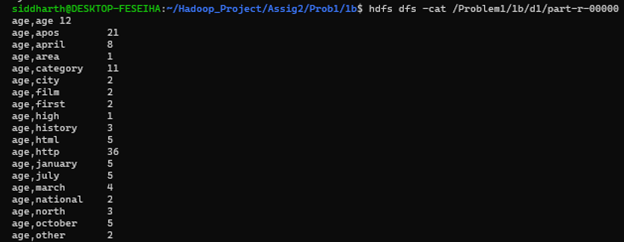
\includegraphics[width=0.85\textwidth]{ScreenShots/Problem1/1b/Pairs_D1.png}
  \caption{Pairs approach, $d = 1$ (small case)}
\end{figure}
\begin{figure}[H]
  \centering
  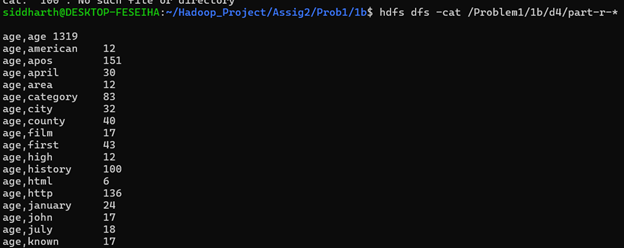
\includegraphics[width=0.85\textwidth]{ScreenShots/Problem1/1b/Pairs_D4.png}
  \caption{Pairs approach, $d = 4$ (largest case)}
\end{figure}

% ───────────────────────────────────────────────────────────
\subsection{Part (c): Co-Occurring Word Matrix -- Stripes Approach}

\subsubsection{Program Logic}

The Stripes approach optimizes the co-occurrence matrix generation by grouping neighbor counts into an associative array (stripe) before emitting them from the Mapper.

\begin{itemize}
    \item \textbf{Setup Phase}: Similar to the Pairs approach, the top-50 words are loaded into a \texttt{HashSet} from the \textit{Distributed Cache}. The configurable window distance $d$ is retrieved from the environment settings.
    \item \textbf{Mapper}: For each word $w_i$ in the input text that belongs to the top-50 set, the Mapper creates a local map (stripe). It scans the next $d$ words; for any neighbor $w_j$ also in the top-50 set, it increments the count for $w_j$ within the stripe. Finally, it emits $w_i$ as the key and the entire stripe as the value.
    \item \textbf{Reducer}: Receives a word $w_i$ and a collection of stripes. It merges all these associative arrays by summing the counts for each individual neighbor across all stripes. This results in a single, consolidated stripe representing all co-occurrences for that specific word.
\end{itemize}

\subsubsection{Pseudocode}

\begin{lstlisting}[style=pseudocode, caption={Co-occurring Word Matrix -- Stripes Approach}]
// Setup: load top-50 words and distance d
function setup(context):
    top50 = load_top_words_from_cache()
    d = get_config("distance")

// Mapper
function Map(key, line):
    tokens = line.toLowerCase().split()
    for i = 0 to tokens.length - 1:
        w1 = tokens[i]
        if w1 in top50:
            stripe = {} // Associative array
            for j = i + 1 to min(i + d, tokens.length - 1):
                w2 = tokens[j]
                if w2 in top50:
                    stripe[w2] += 1
            if stripe is not empty:
                emit(w1, stripe)

// Reducer
function Reduce(word, stripes):
    merged_stripe = {}
    for each stripe in stripes:
        for each (neighbor, count) in stripe:
            merged_stripe[neighbor] += count
    emit(word, merged_stripe)
\end{lstlisting}

\subsubsection{Runtime Analysis for $d \in \{1, 2, 3, 4\}$}

\begin{table}[H]
  \centering
  \caption{Stripes Approach -- Runtime for varying word distance $d$}
  \label{tab:stripes_runtime}
  \renewcommand{\arraystretch}{1.4}
  \begin{tabular}{>{\bfseries}c ccc}
    \toprule
    \rowcolor{lightblue}
    \textbf{Distance $d$} & \textbf{Real Time} & \textbf{User Time} & \textbf{Sys Time} \\
    \midrule
    1 & 1m31.684s & 1m39.614s & 0m10.104s \\
    2 & 1m38.362s & 1m51.021s & 0m10.491s \\
    3 & 1m49.707s & 1m59.632s & 0m10.749s \\
    4 & 3m14.572s & 3m33.349s & 0m21.066s \\
    \bottomrule
  \end{tabular}
\end{table}

\begin{infobox}
  \textbf{Runtime Behavior with Increasing Window Size:} \\
  From the experimental results, it is observed that the runtime increases steadily as the word distance ($d$) increases. The execution time is lowest at $d = 1$ and gradually rises for $d = 2$ and $d = 3$, with a significant spike at $d = 4$. This indicates that larger window sizes introduce higher computational and processing overhead in the stripes approach.
  \vspace{0.5em}

  \textbf{Impact of Stripes-Based Aggregation:} \\
  In the stripes approach, each word is associated with a map (stripe) containing its neighboring words. As the window size increases, the number of neighbors per word also increases, leading to larger stripe sizes. While this reduces the number of intermediate key-value pairs, it significantly increases memory usage and computation required to manage these larger data structures.
  \vspace{0.5em}

  \textbf{Effect on System Performance:} \\
  This overhead becomes particularly noticeable at higher values of $d$, where both user time and system time increase sharply, reflecting the cost of handling larger in-memory structures and increased data processing.
  \vspace{0.5em}

  \textbf{Conclusion:} \\
  Unlike earlier observations, the stripes approach does not always benefit from larger window sizes. While it reduces intermediate data emission, the overhead of maintaining large stripes outweighs these benefits at higher values of $d$. As a result, smaller window sizes provide better performance, and very large window sizes lead to significant performance degradation.
\end{infobox}
\subsubsection{Selected Output Cases -- Stripes Approach}

\begin{infobox}
  \textbf{Representative Results:} \\
  We show the smallest window case ($d = 1$) and the largest window case ($d = 4$) for the Pairs approach. The complete result set for $d \in \{1,2,3,4\}$ is available in the GitHub folder: \texttt{Problem1b}.
\end{infobox}
\begin{figure}[H]
  \centering
  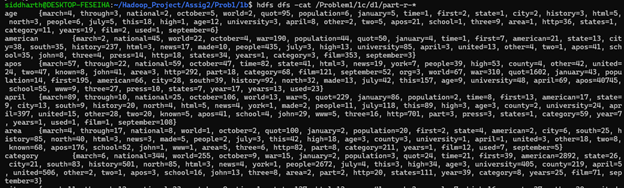
\includegraphics[width=0.85\textwidth,height=4cm]{ScreenShots/Problem1/1c/Stripes_D1.png}
  \caption{Stripes approach, $d = 1$ (small case)}
\end{figure}
\begin{figure}[H]
  \centering
  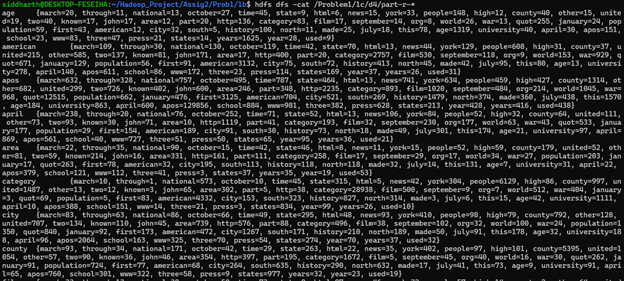
\includegraphics[width=0.85\textwidth]{ScreenShots/Problem1/1c/Stripes_D4.png}
  \caption{Stripes approach, $d = 4$ (largest case)}
\end{figure}
\subsubsection{Pairs vs.\ Stripes -- Comparison}

\begin{infobox}
  \textbf{Runtime Comparison: Pairs vs Stripes Approach} \\
  From the experimental results, it is observed that both the pairs and stripes approaches exhibit increasing runtime with larger window sizes ($d$), but their behavior differs in terms of scalability and overhead.
  \vspace{0.5em}
  
  \textbf{Performance at Smaller Window Sizes} \\
  For smaller values of $d$ (1 and 2), the pairs approach performs slightly better than the stripes approach. The number of co-occurring pairs is relatively limited, and the overhead of maintaining complex stripe data structures in the stripes approach outweighs its benefits.
  \vspace{0.5em}
  
  \textbf{Behavior at Larger Window Sizes} \\
  As the window size increases, both approaches experience higher runtime due to increased computational and data processing requirements. However, the nature of the increase differs:
  \begin{itemize}
    \item In the pairs approach, runtime increases significantly at $d = 3$ because the large number of emitted key-value pairs leads to higher shuffle and communication overhead.
    \item In the stripes approach, runtime increases more gradually up to $d = 3$, but shows a sharp spike at $d = 4$ due to the overhead of managing very large stripe structures in memory.
  \end{itemize}
  \vspace{0.5em}
  
  \textbf{Conclusion} \\
  Overall, the pairs approach is more efficient for smaller window sizes due to its simpler data structures, while the stripes approach can offer better performance at moderate window sizes by reducing shuffle overhead. However, for very large window sizes, both approaches suffer from performance degradation, with stripes being more affected because of increased memory and computation overhead.
\end{infobox}

\subsubsection{Comparison Graph}

\begin{figure}[H]
  \centering
  
\includegraphics[width=0.85\textwidth]{pairs_vs_stripes_runtime.png}
  \caption{Runtime comparison between Pairs and Stripes approaches for varying window sizes.}
  \label{fig:pairs_vs_stripes}
\end{figure}


% ───────────────────────────────────────────────────────────
\subsection{Part (e): Local Aggregation Comparison }

\begin{infobox}
  \textbf{Overview:} Local aggregation is implemented at two levels -- \textbf{Map-function level} (in-mapper combining) and \textbf{Map-class level} (using Hadoop's Combiner class). Both are evaluated for the Pairs and Stripes approaches across $d \in \{1,2,3,4\}$.
\end{infobox}

% ── 1e-i ──────────────────────────────────────────────────
\subsubsection{Local Aggregation -- Program Logic}

Local aggregation is a technique to reduce the volume of data shuffled across the network by combining intermediate results on the Mapper node.

\begin{itemize}
    \item \textbf{Map-Function Level Aggregation}: A local hash map is instantiated inside the \texttt{map()} function. It aggregates co-occurrences found within a single record (input line). The aggregated counts are emitted to the framework at the end of each \texttt{map()} call. This approach provides fine-grained reduction but does not share state across different records.
    \item \textbf{Map-Class Level Aggregation (In-Mapper Combining)}: A global hash map is maintained as a class instance variable. It is initialized once in the \texttt{setup()} method and updated by every \texttt{map()} call in the task. The final aggregated counts are emitted only once during the \texttt{cleanup()} phase. This is more efficient as it combines data across the entire input split assigned to the Mapper.
    \item \textbf{Pairs vs. Stripes Local Aggregation}: For the Pairs approach, local aggregation combines identical pair keys. For the Stripes approach, local aggregation merges multiple stripes for the same primary word, effectively performing a mini-reduction of associative arrays before they leave the Mapper.
\end{itemize}

\subsubsection{Pseudocode-Pairs}

% ── 1e-ii ─────────────────────────────────────────────────
\begin{lstlisting}[style=pseudocode, caption={Map-Function Level Local Aggregation}]
function Map(key, line):
    local_counts = {} // Initialized inside function
    words = tokenize(line)
    for i = 0 to words.length - 1:
        for j = i + 1 to min(i + d, words.length - 1):
            local_counts[(words[i], words[j])] += 1
    
    // Emit results for THIS map call
    for each (pair, count) in local_counts:
        emit(pair, count)
\end{lstlisting}



\begin{lstlisting}[style=pseudocode, caption={Map-Class Level Local Aggregation}]
// State maintained across map() calls
globalMap = {} // Class instance variable

function setup(context):
    globalMap = {} // Initialized once per task

function Map(key, line):
    words = tokenize(line)
    for i = 0 to words.length - 1:
        for j = i + 1 to min(i + d, words.length - 1):
            globalMap[(words[i], words[j])] += 1

function cleanup(context):
    // Emit cumulative results for the ENTIRE task
    for each (pair, count) in globalMap:
        emit(pair, count)
\end{lstlisting}
\subsubsection{Pseudocode-Stripes}

\begin{lstlisting}[style=pseudocode, caption={Map-Function Level Local Aggregation -- Stripes}]
function Map(key, line):
    localStripes = {} // Map<Word, Stripe> (per record)
    words = tokenize(line)
    for i = 0 to words.length - 1:
        if words[i] in top50:
            for j = i + 1 to min(i+d, words.length - 1):
                if words[j] in top50:
                    localStripes[words[i]][words[j]] += 1
    
    // Emit results for THIS record
    for each (word, stripe) in localStripes:
        emit(word, stripe)
\end{lstlisting}

\begin{lstlisting}[style=pseudocode, caption={Map-Class Level Local Aggregation -- Stripes (In-Mapper Combining)}]
// State maintained across map() calls
globalStripes = {} // Map<Word, Stripe>

function setup(context):
    globalStripes = {}

function Map(key, line):
    words = tokenize(line)
    for i = 0 to words.length - 1:
        if words[i] in top50:
            for j = i + 1 to min(i+d, words.length - 1):
                if words[j] in top50:
                    globalStripes[words[i]][words[j]] += 1

function cleanup(context):
    // Emit cumulative stripes for the ENTIRE task
    for each (word, stripe) in globalStripes:
        emit(word, stripe)
\end{lstlisting}

\subsubsection{Pairs Approach -- Local Aggregation Runtime Comparison}
% ── 1e-iii -- PAIRS tables ─────────────────────────────────
\begin{table}[H]
  \centering
  \caption{Pairs -- Map-Function Level Aggregation Runtime}
  \label{tab:pairs_fn_agg}
  \renewcommand{\arraystretch}{1.4}
  \begin{tabular}{>{\bfseries}c ccc}
    \toprule
    \rowcolor{lightblue}
    \textbf{Distance $d$} & \textbf{Real Time} & \textbf{User Time} & \textbf{Sys Time} \\
    \midrule
    1 & 2m58.455s & 2m42.638s & 0m21.392s \\
    2 & 3m38.643s & 4m14.404s & 0m23.974s \\
    3 & 2m51.831s & 3m28.939s & 0m20.737s \\
    4 & 2m10.394s & 2m25.423s & 0m17.873s \\
    \bottomrule
  \end{tabular}
\end{table}

\begin{table}[H]
  \centering
  \caption{Pairs -- Map-Class Level Aggregation Runtime}
  \label{tab:pairs_cls_agg}
  \renewcommand{\arraystretch}{1.4}
  \begin{tabular}{>{\bfseries}c ccc}
    \toprule
    \rowcolor{lightblue}
    \textbf{Distance $d$} & \textbf{Real Time} & \textbf{User Time} & \textbf{Sys Time} \\
    \midrule
    1 & 1m33.533s & 1m48.284s & 0m11.218s \\
    2 & 1m32.204s & 1m45.605s & 0m9.785s \\
    3 & 4m10.047s & 4m40.957s & 0m19.640s \\
    4 & 3m20.290s & 3m34.725s & 0m22.398s \\
    \bottomrule
  \end{tabular}
\end{table}

% ── 1e-iv -- STRIPES tables ────────────────────────────────
\subsubsection{Stripes Approach -- Local Aggregation Runtime Comparison}

\begin{table}[H]
  \centering
  \caption{Stripes -- Map-Function Level Aggregation Runtime}
  \label{tab:stripes_fn_agg}
  \renewcommand{\arraystretch}{1.4}
  \begin{tabular}{>{\bfseries}c ccc}
    \toprule
    \rowcolor{lightblue}
    \textbf{Distance $d$} & \textbf{Real Time} & \textbf{User Time} & \textbf{Sys Time} \\
    \midrule
    1 & 1m38.217s & 1m50.191s & 0m10.000s \\
    2 & 1m42.627s & 2m0.027s & 0m11.174s \\
    3 & 2m19.048s & 2m45.673s & 0m20.009s \\
    4 & 5m6.088s & 5m36.322s & 0m32.163s \\
    \bottomrule
  \end{tabular}
\end{table}

\begin{table}[H]
  \centering
  \caption{Stripes -- Map-Class Level Aggregation Runtime}
  \label{tab:stripes_cls_agg}
  \renewcommand{\arraystretch}{1.4}
  \begin{tabular}{>{\bfseries}c ccc}
    \toprule
    \rowcolor{lightblue}
    \textbf{Distance $d$} & \textbf{Real Time} & \textbf{User Time} & \textbf{Sys Time} \\
    \midrule
    1 & 1m48.690s & 1m58.584s & 0m11.933s \\
    2 & 1m39.162s & 2m0.742s & 0m12.899s \\
    3 & 1m22.277s & 1m28.057s & 0m9.536s \\
    4 & 1m46.343s & 2m4.352s & 0m12.471s \\
    \bottomrule
  \end{tabular}
\end{table}

\subsubsection{Selected Output Cases -- Local Aggregation}

\begin{infobox}
  \textbf{Representative Results:} \\
  The following cases are shown for local aggregation at $d = 3$: Pairs Map-Function, Pairs Map-Class, Stripes Map-Function, and Stripes Map-Class. The complete set of local aggregation results is available in the GitHub folder: \texttt{Problem1d}.
\end{infobox}

\begin{figure}[H]
  \centering
  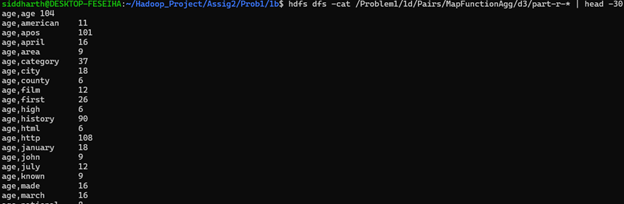
\includegraphics[width=0.85\textwidth]{ScreenShots/Problem1/1d/Pairs/MapFunctionLevelAgg/D3.png}
  \caption{Pairs Map-Function aggregation, $d = 3$}
\end{figure}
\begin{figure}[H]
  \centering
  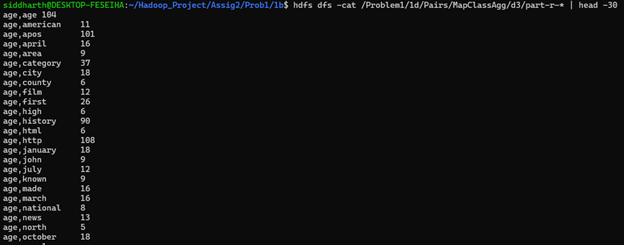
\includegraphics[width=0.85\textwidth]{ScreenShots/Problem1/1d/Pairs/MapClassLevelAgg/D3.png}
  \caption{Pairs Map-Class aggregation, $d = 3$}
\end{figure}

\begin{figure}[H]
  \centering
  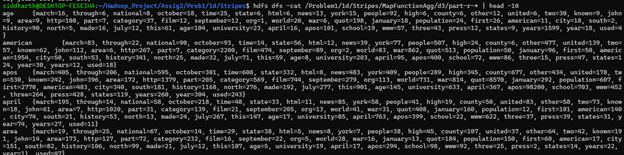
\includegraphics[width=0.85\textwidth]{ScreenShots/Problem1/1d/Stripes/MapClassLevelAgg/D3.png}
  \caption{Stripes Map-Function aggregation, $d = 3$}
\end{figure}
\begin{figure}[H]
  \centering
  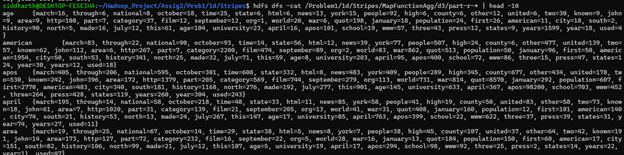
\includegraphics[width=0.85\textwidth]{ScreenShots/Problem1/1d/Stripes/MapClassLevelAgg/D3.png}
  \caption{Stripes Map-Class aggregation, $d = 3$}
\end{figure}

% ── 1e-v -- Summary comparison ─────────────────────────────
\subsubsection{Summary: Performance Comparison Across All Variants}

% \begin{table}[H]
%   \centering
%   \caption{Consolidated Runtime Summary -- All Approaches (Real Time, seconds)}
%   \label{tab:summary_p1}
%   \renewcommand{\arraystretch}{1.5}
%   \begin{tabularx}{\linewidth}{>{\bfseries}c X X X X X}
%     \toprule
%     \rowcolor{lightblue}
%     \textbf{$d$}
%       & \textbf{Pairs Base}
%       & \textbf{Pairs Fn-Agg}
%       & \textbf{Pairs Cls-Agg}
%       & \textbf{Stripes Base}
%       & \textbf{Stripes Fn-Agg}
%       \\
%     \midrule
%     1 & \ph{fill} & \ph{fill} & \ph{fill} & \ph{fill} & \ph{fill} \\
%     2 & \ph{fill} & \ph{fill} & \ph{fill} & \ph{fill} & \ph{fill} \\
%     3 & \ph{fill} & \ph{fill} & \ph{fill} & \ph{fill} & \ph{fill} \\
%     4 & \ph{fill} & \ph{fill} & \ph{fill} & \ph{fill} & \ph{fill} \\
%     \bottomrule
%   \end{tabularx}
% \end{table}

\begin{infobox}
  \textbf{1. Pairs: Map-Function vs.\ Map-Class Aggregation}
  \vspace{0.5em}
  
  \textbf{Performance Improvement:} \\
  From the experimental results, it is clearly observed that map-class level aggregation significantly outperforms map-function level aggregation in the pairs approach.
  \vspace{0.5em}
  
  \textbf{For all values of $d$:} \\
  The real execution time of the map-class approach is substantially lower than that of the map-function approach. For instance, at $d = 1$, the runtime reduces from approximately 2m58s (map-function) to 1m33s (map-class), demonstrating a major improvement.
  \vspace{0.5em}
  
  \textbf{Why it works:} \\
  Map-class aggregation accumulates intermediate results across multiple map calls before emitting them. As a result, the number of intermediate key-value pairs is drastically reduced, leading to lower shuffle overhead and improved reducer efficiency.
  \vspace{0.5em}
  
  \textbf{Map-function limitation:} \\
  Map-function aggregation operates at a finer granularity, limiting its ability to effectively reduce intermediate emissions. This results in higher communication overhead and longer execution time.
\end{infobox}

\begin{infobox}
  \textbf{2. Stripes: Map-Function vs.\ Map-Class Aggregation}
  \vspace{0.5em}
  
  \textbf{Impact of Aggregation Strategy:} \\
  In the stripes approach, the impact of aggregation strategy is not straightforward.
  \vspace{0.5em}
  
  \textbf{Observed behavior:} \\
  While map-function aggregation performs reasonably well for smaller values of $d$, its performance degrades significantly as $d$ increases, particularly at $d = 4$, where the runtime rises sharply to over 5 minutes. This is due to the increasing size of stripes, which leads to higher memory usage and computational overhead.
  \vspace{0.5em}
  
  \textbf{Stable performance with map-class:} \\
  Map-class aggregation provides more stable and efficient performance across all values of $d$. Notably, at $d = 3$, it achieves the best performance (1m22s), significantly outperforming the map-function approach.
  \vspace{0.5em}
  
  \textbf{What it implies:} \\
  This indicates that map-class aggregation is more effective in managing large stripe structures by reducing redundant emissions and improving data locality.
\end{infobox}

\begin{infobox}
  \textbf{3. Effect of Local Aggregation \& Overall Comparison}
  \vspace{0.5em}
  
  \textbf{Performance Role of Local Aggregation:} \\
  Local aggregation plays a critical role in improving performance, particularly in the pairs approach. By reducing the number of intermediate key-value pairs emitted by the mapper, it minimizes shuffle and network overhead, which are major bottlenecks in MapReduce jobs.
  \vspace{0.5em}
  
  \textbf{Pairs Approach Benefit:} \\
  In the pairs approach, local aggregation leads to substantial performance gains, with map-class aggregation emerging as the most efficient strategy.
  \vspace{0.5em}
  
  \textbf{Stripes Approach Benefit:} \\
  In the stripes approach, although local aggregation still provides benefits, the improvements are less dramatic. This is because the stripes approach inherently performs aggregation by grouping neighboring words into a single data structure. However, at larger window sizes, the overhead of managing large stripes dominates performance, especially in the absence of efficient aggregation.
\end{infobox}

\subsubsection{Performance Comparison Graphs}

\begin{figure}[H]
    \centering
    \setlength{\fboxsep}{5pt}
    
    \fbox{
\includegraphics[width=0.8\textwidth]{pairs_local_agg.png}}
    \caption{Pairs Approach: Map-Function vs.\ Map-Class}
    
    \vspace{0.5cm}
    
    \fbox{
\includegraphics[width=0.8\textwidth]{stripes_local_agg.png}}
    \caption{Stripes Approach: Map-Function vs.\ Map-Class}
    
\end{figure}

\newpage

% ╔══════════════════════════════════════════════════════════╗
% ║         PROBLEM 2 -- INDEXING DOCUMENTS VIA HADOOP       ║
% ╚══════════════════════════════════════════════════════════╝
\section{Problem 2: Indexing Documents via Hadoop}

\begin{infobox}
  \textbf{Objective:} Compute Document Frequency (DF) for all terms in the Wikipedia corpus, then compute a TF-IDF–style score for the top-100 high-DF terms across all documents. The Porter Stemmer from \texttt{opennlp-tools-1.9.3.jar} is used for term normalisation.
\end{infobox}

% ───────────────────────────────────────────────────────────
\subsection{Part (a): Document Frequency Computation}

\subsubsection{Program Logic}

The Document Frequency (DF) program identifies the total number of documents (or records) in which each unique term appears across the Wikipedia corpus. Term normalization via stemming is employed to aggregate variations of the same root word.

\begin{itemize}
    \item \textbf{Setup Phase}: The stopwords file is loaded from the \textit{Distributed Cache} into a \texttt{HashSet} in the Mapper's \texttt{setup()} method. A \texttt{PorterStemmer} instance is also created for term normalization.
    \item \textbf{Mapper}: The mapper derives a document ID from the input filename by stripping the file extension. Each input line is converted to lowercase, split on non-alphabetic characters, and filtered for valid tokens (length > 2, alphabetic, not Roman numerals). Stopwords are removed before and after stemming. A per-line \texttt{HashSet} ensures each stemmed term is emitted at most once per line. The mapper emits \texttt{(stemmed	erm, docId)} for each distinct term.
    \item \textbf{Reducer}: For each stemmed term, the reducer collects all document IDs, deduplicates them using a \texttt{HashSet}, and writes the term with its distinct document frequency count. This produces the final DF values for the corpus.
    \item \textbf{Post-processing}: The resulting TSV is sorted numerically by DF in descending order using shell commands to identify the top-100 terms.
\end{itemize}

\subsubsection{Pseudocode}

\begin{lstlisting}[style=pseudocode, caption={Document Frequency -- Map and Reduce}]
// Setup: load stopwords and initialize stemmer
function setup(context):
    stopwords = load_from_cache()
    stemmer = new PorterStemmer()

// Mapper
function Map(filePath, line):
    docId = extract_filename_without_extension(filePath)
    tokens = tokenize(line.toLowerCase())
    seenThisLine = {}

    for each token in tokens:
        if not isValidToken(token):
            continue
        if token in stopwords:
            continue
        stemmed = stemmer.stem(token)
        if not isValidToken(stemmed):
            continue
        if stemmed in stopwords:
            continue
        if stemmed not in seenThisLine:
            seenThisLine.add(stemmed)
            emit(stemmed, docId)

// Reducer
function Reduce(term, docIds):
    distinctDocs = {}
    for each docId in docIds:
        distinctDocs.add(docId)
    emit(term, size(distinctDocs))
\end{lstlisting}

\subsubsection{Post-processing for Top-100 Terms}

The following shell command extracts the top-100 highest document-frequency terms by sorting the MapReduce output:

\begin{lstlisting}[style=bashcode]
hdfs dfs -cat /problem2/2a/df.tsv | sort -k2 -nr | head -100 > top100.txt
\end{lstlisting}
\subsubsection{Runtime Analysis}

\begin{infobox}
  \runtime{1m56.062s}{2m11.019s}{0m9.638s}
  \vspace{0.5em}
\end{infobox}

\begin{infobox}
  \textbf{Runtime Behavior} \\
  The execution time for document frequency computation is observed to be approximately 1 minute and 56 seconds. The user time (2 minutes and 11 seconds) is higher than the real time, indicating that multiple map and reduce tasks are executing in parallel, resulting in CPU usage exceeding the wall-clock time.
  \vspace{0.5em}

  \textbf{Computation vs Framework Overhead} \\
  The relatively high user time reflects the computational complexity involved in tokenization, stopword removal, stemming, and tracking unique document occurrences for each term. These operations require significant CPU processing across multiple nodes or threads.
  \vspace{0.5em}

  \textbf{Parallelism Effect} \\
  At the same time, the difference between real time and user time suggests that Hadoop effectively utilizes parallelism to distribute the workload.
  \vspace{0.5em}

  \textbf{System Overhead} \\
  The system time remains relatively low (around 9 seconds), indicating that operating system-level operations such as file handling and process management do not contribute significantly to the overall execution time.
\end{infobox}

\subsubsection{Output Schema}

The output TSV file has the following schema:
\begin{center}
  \texttt{TERM\textbackslash tDF}
\end{center}

\subsubsection{Top-100 High Document Frequency Terms}
\begin{figure}[H]
  \centering
  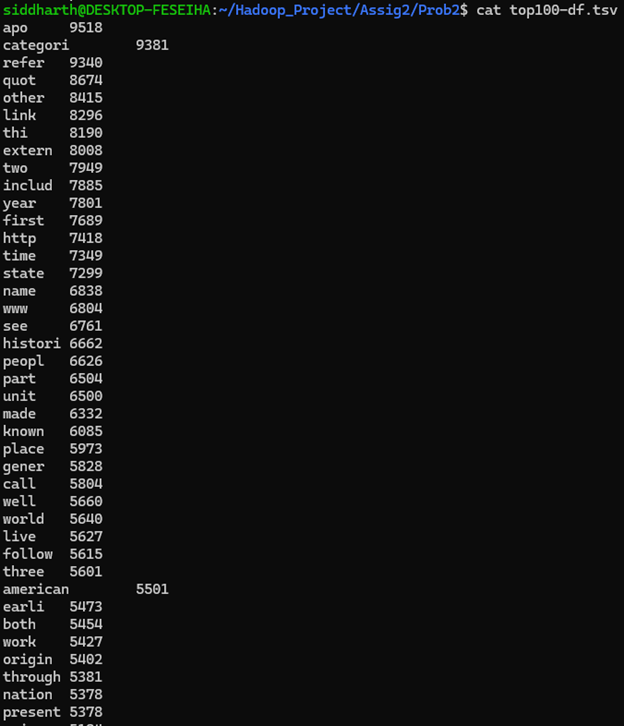
\includegraphics[width=0.85\textwidth]{ScreenShots/Problem2/Top100DF.png}
  \caption{Pairs Map-Function aggregation, $d = 3$}
\end{figure}


% ───────────────────────────────────────────────────────────
\subsection{Part (b): TF-IDF Score Computation -- Stripes Approach}

\subsubsection{Program Logic}

The Stripes approach is used to efficiently compute the TF-IDF scores for the top-100 high-DF terms across Wikipedia documents.

\begin{itemize}
    \item \textbf{Setup Phase}: Both the Mapper and the Reducer load the \texttt{df\_top100.tsv} file from the \textit{Distributed Cache}. This populates a \texttt{dfMap} in each task, containing only the top-100 terms and their document frequencies.
    \item \textbf{Mapper}: The mapper derives the document ID from the input filename by stripping the file extension. For each input line, it tokenizes and lowercases text, stems each token, and checks whether the stemmed term is in \texttt{dfMap}. If so, it increments the count in an in-memory stripe for that document. No output is emitted inside \texttt{map()}; instead, the mapper emits one stripe per document during \texttt{cleanup()}.
    \item \textbf{Stripe Format}: Each emitted stripe is serialized as a string of the form \texttt{term1:count1|term2:count2|...}, where \texttt{|} separates term-count pairs and \texttt{:} separates term and count.
    \item \textbf{Reducer}: For each document ID, the reducer receives one or more stripe strings. It merges these partial stripes into a single term-count map, computes TF-IDF scores using \texttt{SCORE = TF * log(10000 / DF + 1)}, and emits output in the schema \texttt{docId\tterm\tscore}.
\end{itemize}

\subsubsection{Scoring Formula}

\[
  \text{SCORE}(t, d)
    = \text{TF}(t, d) \times \log\!\left(\frac{10000}{\text{DF}(t)} + 1\right)
\]

where $\text{TF}(t, d)$ is the count of term $t$ in document $d$, and $\text{DF}(t)$ is the number of distinct documents containing $t$ across the entire corpus.

\subsubsection{Pseudocode}

\begin{lstlisting}[style=pseudocode, caption={TF-IDF Score -- Stripes MapReduce}]
// Setup: load DF map from Distributed Cache (Mapper & Reducer)
function setup(context):
    df_map = load_tsv_as_map(cache_file) // Maps term -> DF

// Mapper (Stripes)
function Map(filePath, line):
    docID = extract_filename_without_extension(filePath)
    stripe = docStripes[docID] if exists else {}
    tokens = tokenize(line.toLowerCase())
    for each token in tokens:
        stemmed = stem(token)
        if stemmed in df_map:
            stripe[stemmed] += 1
    docStripes[docID] = stripe

function cleanup(context):
    for each (docID, stripe) in docStripes:
        stripeString = serialize_stripe(stripe)  // term:count|term:count|...
        emit(docID, stripeString)

// Reducer
function Reduce(docID, stripeStrings):
    termCounts = {}
    for each stripeString in stripeStrings:
        pairs = split(stripeString, "|")
        for each pair in pairs:
            (term, count) = split(pair, ":")
            termCounts[term] += parseInt(count)

    for each (term, tf) in termCounts:
        df = df_map[term]
        score = tf * log(10000.0 / df + 1)
        emit(docID, term + "\t" + format(score, 6))
\end{lstlisting}


\subsubsection{Runtime Analysis}

\begin{infobox}
  \runtime{0m52.046s}{0m59.602s}{0m6.379s}
\end{infobox}

\begin{infobox}
  \textbf{Runtime Behavior:} \\
  The execution time for TF-IDF score computation is observed to be approximately 52 seconds, which is significantly lower than that of document frequency computation. This improvement is primarily because document frequency operates on the entire vocabulary of the dataset, whereas TF-IDF is restricted to a smaller subset of top-100 terms, thereby reducing the input size and computational workload.
  \vspace{0.5em}
  
  \textbf{Efficiency of Stripes Approach:} \\
  The use of the stripes approach enables efficient aggregation of term frequencies, minimizing the number of intermediate key-value pairs and reducing shuffle overhead. The user time (59 seconds) is slightly higher than the real time (52 seconds), indicating that multiple MapReduce tasks are executed in parallel, leading to cumulative CPU usage exceeding the wall-clock time.
\end{infobox}

\subsubsection{Output Schema}

The output TSV file has the following schema:
\begin{center}
  \texttt{ID\textbackslash tTERM\textbackslash tSCORE}
\end{center}

The \texttt{ID} field uses dynamically generated integer IDs derived from the byte offset of the record (e.g., \texttt{DOC\_12345}).

\subsubsection{Representative TF-IDF Output}
\begin{figure}[H]
  \centering
  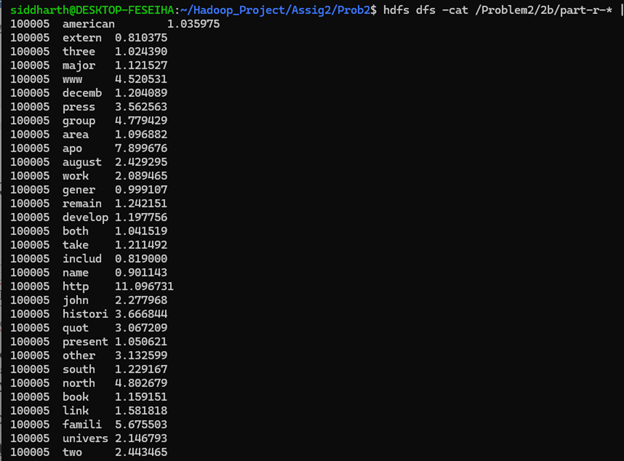
\includegraphics[width=0.85\textwidth]{ScreenShots/Problem2/TFIDF_Scores.png}
  \caption{TF-IDF Output }
\end{figure}


\newpage

% ╔══════════════════════════════════════════════════════════╗
% ║                    APPENDIX                             ║
% ╚══════════════════════════════════════════════════════════╝
\section*{Appendix}
\addcontentsline{toc}{section}{Appendix}

\subsection*{A. System Configuration}

\begin{table}[H]
  \centering
  \renewcommand{\arraystretch}{1.4}
  \begin{tabular}{ll}
    \toprule
    \textbf{Parameter} & \textbf{Value} \\
    \midrule
    Hadoop Ver. & 3.4.3 \\
    Java Ver.   & Java 8 \\
    Dataset     & Wikipedia-EN-20120601\_ARTICLES.tar.gz \\
    Testing Dataset     & Wikipedia-50-Articles.tar \\
    \bottomrule
  \end{tabular}
  \caption{Experimental System Configuration}
\end{table}

\subsection*{B. Run Instructions}

\begin{itemize}[nosep]
  \item \texttt{problem\_1.txt} -- Instructions for Problem 1 (parts a, b, c, e)
  \item \texttt{problem\_2.txt} -- Instructions for Problem 2 (parts a, b)
\end{itemize}

The solution is submitted in a ZIP file, and the same contents are also available in the GitHub repository linked with this assignment.



\subsection*{D. Shared Tokenization and Normalization}

The tokenization logic is kept consistent across all MapReduce implementations in this assignment. Each line is converted to lowercase and split using the regular expression \verb|[^a-z]+|, which removes every non-alphabetic separator. After splitting, tokens are filtered to remove:

\begin{itemize}
    \item tokens of length two or less,
    \item non-alphabetic tokens,
    \item Roman numerals (e.g., \texttt{i}, \texttt{ii}, \texttt{iii}), and
    \item stopwords loaded from \texttt{stopwords.txt} via the distributed cache.
\end{itemize}

The remaining tokens are then stemmed using the OpenNLP Porter stemmer before further processing. This shared normalization ensures consistent term matching across both Problem 1 and Problem 2 implementations.

\end{document}
  